\hypertarget{group__x_event_group_clear_bits_from_i_s_r}{}\section{x\+Event\+Group\+Clear\+Bits\+From\+I\+SR}
\label{group__x_event_group_clear_bits_from_i_s_r}\index{x\+Event\+Group\+Clear\+Bits\+From\+I\+SR@{x\+Event\+Group\+Clear\+Bits\+From\+I\+SR}}
Collaboration diagram for x\+Event\+Group\+Clear\+Bits\+From\+I\+SR\+:\nopagebreak
\begin{figure}[H]
\begin{center}
\leavevmode
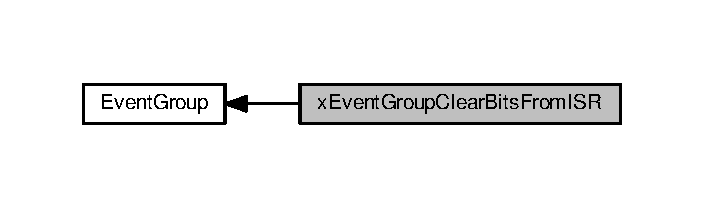
\includegraphics[width=338pt]{group__x_event_group_clear_bits_from_i_s_r}
\end{center}
\end{figure}
\hyperlink{event__groups_8h}{event\+\_\+groups.\+h} 
\begin{DoxyPre}
   BaseType\_t \hyperlink{event__groups_8h_a3d7de214a697f33fe7b914e26a93f33a}{xEventGroupClearBitsFromISR( EventGroupHandle\_t xEventGroup, const EventBits\_t uxBitsToSet )};
\end{DoxyPre}


A version of \hyperlink{event__groups_8h_a0fb72cfdd4f0d5f86d955fc3af448f2a}{x\+Event\+Group\+Clear\+Bits()} that can be called from an interrupt.

Setting bits in an event group is not a deterministic operation because there are an unknown number of tasks that may be waiting for the bit or bits being set. Free\+R\+T\+OS does not allow nondeterministic operations to be performed while interrupts are disabled, so protects event groups that are accessed from tasks by suspending the scheduler rather than disabling interrupts. As a result event groups cannot be accessed directly from an interrupt service routine. Therefore \hyperlink{event__groups_8h_a3d7de214a697f33fe7b914e26a93f33a}{x\+Event\+Group\+Clear\+Bits\+From\+I\+S\+R()} sends a message to the timer task to have the clear operation performed in the context of the timer task.


\begin{DoxyParams}{Parameters}
{\em x\+Event\+Group} & The event group in which the bits are to be cleared.\\
\hline
{\em ux\+Bits\+To\+Clear} & A bitwise value that indicates the bit or bits to clear. For example, to clear bit 3 only, set ux\+Bits\+To\+Clear to 0x08. To clear bit 3 and bit 0 set ux\+Bits\+To\+Clear to 0x09.\\
\hline
\end{DoxyParams}
\begin{DoxyReturn}{Returns}
If the request to execute the function was posted successfully then pd\+P\+A\+SS is returned, otherwise pd\+F\+A\+L\+SE is returned. pd\+F\+A\+L\+SE will be returned if the timer service queue was full.
\end{DoxyReturn}
Example usage\+: 
\begin{DoxyPre}
  #define BIT\_0 ( 1 << 0 )
  #define BIT\_4 ( 1 << 4 )\end{DoxyPre}



\begin{DoxyPre}  // An event group which it is assumed has already been created by a call to
  // xEventGroupCreate().
  EventGroupHandle\_t xEventGroup;\end{DoxyPre}



\begin{DoxyPre}  void anInterruptHandler( void )
  \{
    // Clear bit 0 and bit 4 in xEventGroup.
    xResult = xEventGroupClearBitsFromISR(
                        xEventGroup,     // The event group being updated.
                        BIT\_0 | BIT\_4 ); // The bits being set.\end{DoxyPre}



\begin{DoxyPre}    if( xResult == pdPASS )
    \{
        // The message was posted successfully.
    \}
 \}
  \end{DoxyPre}
 